\documentclass[12pt,letterpaper]{article}
\input{../../preamble}
\usepackage{fullpage}
\usepackage{multicol}

\begin{document}
\flushleft
\begin{multicols}{2}
\textbf{Math 2554 Exam 2 \\
Friday 27 February 2015}

%\hfill
\textbf{Name:  }\underline{\hspace{45ex}} %KEY\hspace{17ex}}

\vspace{.5in}

\end{multicols}

\pagestyle{empty}

\flushleft

\begin{center}\LARGE Calculus I 

Exam 2: Derivatives \end{center}

\vspace{1.5pc}
Please provide the following data:

\vspace{1.5pc}
Drill Instructor: \underline{\hspace{40ex}}

\vspace{1.5pc}
Drill Time: \underline{\hspace{40ex}}

\vspace{1.5pc}
Student ID or clicker \#: \underline{\hspace{40ex}}

%\vfill
\vspace{3pc}
{\bf Exam Instructions:} You have 50 minutes to complete this exam.  One $3\times 5$ inch notecard, one side only, is allowed.  No graphing calculators.  No programmable calculators.  No electronic devices except for the approved calculators (so no phones, iDevices, computers, etc).  If you finish early then you may leave, UNLESS there are less than 5 minutes of class left.  To prevent disruption, if you finish with less than 5 minutes of class remaining then please stay seated and quiet.

%\vspace{2pc}
\vfill
\textbf{Your signature below indicates that you have read this page and agree to follow the Academic Honesty Policies of the University of Arkansas.}  

\vspace{2pc}
Signature: {\bf (1 pt)} \underline{\hspace{91ex}}

%\vfill
\begin{flushright}\Large Good luck!\end{flushright}

\begin{enumerate}[1.]
% % % % %	
\newpage
\item {\bf (3 pts each)} For each function $g(x)$, find the value of $g'(3)$ using the data given below.
\begin{align*}
f(1)=6 & \qquad f(3)=2 & f(6)=5 & \qquad f(9)=-3\\
f'(1)=-2 & \qquad f'(3)=4 & f'(6)=-1 & \qquad f'(9)=1
\end{align*}

\vspace{1pc}
	\begin{enumerate}[(a)]
	\item $g(x)=f(3)+10f(2x)$
	
	\vspace{10pc}
	\item $g(x)=\displaystyle\frac{f(x)}{x}$
	
	\vspace{10pc}
	\item $g(x)=\left(f(x)\right)^3$
	
	\vspace{10pc}
	\item {\bf EXTRA CREDIT} $g(x)=f(x^2)$
	\end{enumerate}
	
% % % % %
\newpage
\item {\bf (8 pts)} Evaluate $\displaystyle\lim_{x\to 0}\frac{\sin{3x}}{x}$.

\vspace{21pc}
\item {\bf (5 pts each)} Suppose a company produces $x$ items at a cost $C(x)$.
	\begin{enumerate}[(a)]
	\item Write the formula for {\bf average cost} and say in words what it means.

	\vspace{12pc}		
	\item Write the formula for {\bf marginal cost} and say in words what it means..
	\end{enumerate}

% % % % %
\newpage
\item {\bf (8 pts each)} For each function find $\displaystyle\dfrac{d^2y}{dx^2}$.
	\begin{enumerate}
	\item $x^4+y^4=64$
	
	\vspace{25pc}
	\item $e^{2y}+x=y$
	\end{enumerate}

% % % % %
\newpage	
\item {\bf (4 pts each)} Let $F=f+g$ and $G=3f-g$, where the graphs of $f$ and $g$ are shown in Figure \ref{fig:graphDeriv}.

\vspace{-0.5pc}  
\begin{figure}[h]
\begin{center}
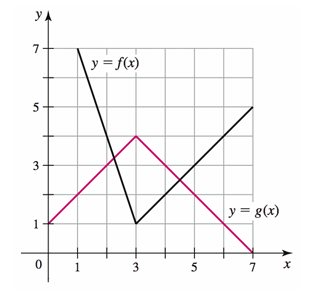
\includegraphics[scale=0.8]{Exam2graphDeriv.png}
\caption{(Briggs, W. and Cochran, L. \emph{Calculus: Early Transcendentals})}
\label{fig:graphDeriv}
\end{center}
\end{figure}

Find the following derivatives:
	\begin{enumerate}[(a)]
	\item $F'(1)$
	
	\vspace{6pc}
	\item $G'(1)$
	
	\vspace{6pc}
	\item $F'(5)$
	
	\vspace{6pc}
	\item $G'(5)$
	\end{enumerate}
		
% % % % % 
\newpage
\item {\bf (3 pts each)} Find the derivative of each of the following functions:
	\begin{enumerate}[(a)]
	\item $\displaystyle f(x)=\frac{(x-1)(2x^2-1)}{x^3-1}$
	
	\vspace{25pc}
	\item $\displaystyle f(x)=\frac{x+1}{x^2e^{2x}}$

% % % % %
\newpage	
	\item $y=\sin x+\cos x$
	
	\vspace{16pc}
	\item $y=5x^2+\cos x$
	
	\vspace{16pc}
	\item $\displaystyle y=\frac{(x^2-1)\sin x}{\sin x+1}$
	\end{enumerate}
\end{enumerate}

% % % % % % % % % %	

\end{document}


